\documentclass[letterpaper]{article}
\usepackage{polyglossia, fontspec}
\usepackage{amsmath, mathtools}
\usepackage[linkcolor=blue, colorlinks=true]{hyperref}
\usepackage{tikz}
\usetikzlibrary{bayesnet}
\usepackage[margin = 1.5 in]{geometry}
\usepackage{multirow}

\title{Binomial Models of Read Counts}
\author{Attila Gulyás-Kovács}
\bibliographystyle{plain}

\begin{document}

\maketitle

\section{Introduction}

\subsection{Goals}

\begin{description}
\item[estimation of \(1-\pi_0\)], where \(\pi_0\) is the genome-wide probability
(i.e.~the expected fraction) of biallelically
expressed genes
\item[within-gene variation] how does exclusion state vary
population-wide within any given gene?
\item[regression] if there is such variation, how is it explained by age and
other measured variables?
\item[classification] predict exclusion state for each individual--gene pair
to learn about species and tissue specificity
\end{description}

To what extent has the previous work achieved these goals?  Estimation of
\(\pi_0\) has not yet been achieved.  Within-gene variation has been
characterized using the conditional distribution of the \(S_{ig}\) statistic
for any given gene \(g\) but it remains unknown what is the relative contribution of within-gene and of
across-gene (genome-wide) variance to the total variance (both across
individuals and genes).  Regression on explanatory variables has been performed but
left the generality and statistical significance of the results an open
question.  Classification has been performed using \(S_{ig}\) but without
estimated error rates and---inconsistently with the results of regression
analysis---also without taking explanatory variables into account.

\subsection{Improvement relative to previous approach}
\label{sec:improvement}

\begin{table}[t]
\begin{tabular}{rr|cc}
& & previous & proposed \\
\hline
\hline
\multirow{3}{*}{local model(s)} & read counts at heteroz.~sites & binomial &
binomial\\
& sites jointly modeled & no & yes \\
& direct biol.~relevance & no & yes \\
\hline
\multirow{3}{*}{global models} & well-defined & no & yes \\
& objective selection possible & no & yes \\
& selection done & inconsistently & not yet \\
\hline
\multirow{1}{*}{\(\pi_0\) } & estimation possible & no & yes \\
\hline
\multirow{2}{*}{regression} & nonlinearity & no & yes \\
& heteroscedasticity & no & yes\\
\hline
\multirow{3}{*}{classification} & test statistic & \(S_{ig}\) & posterior
pr. \\
& likelihood (distrib.)~known & no & yes \\
& sufficiency (given likelihood) & no & yes \\
& error control & no & yes \\
\hline
\end{tabular}
\caption{
Salient properties of previous model(s) and the ones proposed in this article,
and properties of inferences based on those models.
}
\label{tab:previous-proposed}
\end{table}

As explained in this section, answering the remaining questions is limited by
the properties of the previous models and---to even greater extent
perhaps---by their incomplete or implicit description.  This has motivated the
present article, which explicitly describes novel modeling
approaches---contrasting them to the previously used ones---, as well as their
inferential utility towards the remaining goals
(Table~\ref{tab:previous-proposed}).

Both the previous and present approach starts out from modeling read counts at
heterozygous sites as binomial random variables.  However, only the present
approach considers their joint distribution at the level of entities that are
directly relevant to biology: transcripts for a given individual and gene,
population-wide within a given gene, and both population- and genome-wide.
This is achieved via local (transcript level, Section~\ref{sec:local-model})
and global (individual and higher levels, Section~\ref{sec:models}) joint
models of the complete data.

These new models draw direct, and explicit, link between read counts and
allelic exclusion state \(\theta_{ig}\) by enabling likelihood calculations.
The previous approach was both indirect and implicit because it used the
\(S_{ig}\) statistic derived from read counts to describe exclusion state in a
non-probabilistic way since the sampling distribution of \(S_{ig}\) for a
given exclusion state was not specified.  That in turn prevented
likelihood calculations.

Were the likelihoods based on \(S_{ig}\) expressed, they would lack some
information on exclusion state.  This is because \(S_{ig}\) only considers the
proportion of read counts (for one allele) discarding the counts themselves,
which enhance confidence.  Further information is lost by the simplifying
assumption on haplotype phase that all ``higher read counts'' originate from
the same chromosome.  These shortcomings imply that \(S_{ig}\) is not a
sufficient
statistic\footnote{\url{https://en.wikipedia.org/wiki/Sufficient\_statistic}}
for exclusion state.  Although the shortcomings had been recognized earlier,
only partial and post-hoc corrections were employed.  In contrast, proposed
local models operate with counts \emph{per se} and also relax the simplifying
assumption on haplotype by considering all possible \emph{allele
configurations}.  Thus they contain all information on exclusion state and its
likelihood\footnote{Note that, trivially, the likelihood is always a
sufficient statistic}.

The lack of \(S_{ig}\)-based likelihood for exclusion state
prevented the estimation of the error rates of classification and that of
genome-wide probabilities \(\pi\) for those states because the two are
inherently coupled, as explained in an earlier article\footnote{Feb 10, 2016:
Project on Monoallelic Expression: a Statistical View}.  On the other hand,
all proposed global models contain a \(\pi\) parameter vector, which can be
estimated by maximum likelihood based on the complete dataset
(Section~\ref{sec:marginal-likelihood-pi}).  That estimate then can be
combined with likelihood ratios representing the odds that the read count data
support mono vs.~biallelic expression (Section~\ref{sec:classification}). This
yields the posterior probability of monoallelic expression, which naturally
incorporates error.  Alternatively, likelihood ratios can be used on their own
as Bayes factors.  Note that the Neyman-Pearson
lemma\footnote{\url{http://mathworld.wolfram.com/Neyman-PearsonLemma.html}}
guarantees that there do not exist more powerful tests than that based on
likelihood ratios.

Previous regression analysis used the vector \(\mathrm{LOI\_R}_g\) as a
response variable, which was derived from \(S_{ig}\) with a data
transformation step.  Some limitations of \(\mathrm{LOI\_R}_g\) obviously
follow from those of \(S_{ig}\) (discussed above).  More limitations have been
found\footnote{lab-notebook post from Mar 2, 2016: Repeating Ifat's Regression
Analysis with 5 More Genes} to have arisen from the previous incorrect use of
regression weights.  Moreover, the data transformation may introduce biased
estimation of regression parameters due to insufficient removal of the
observed strong nonlinearity and heteroscedasticity of read
count/\(S_{ig}\)-based regression.  Finally, the interpretation of
\(\mathrm{LOI\_R}_g\)-based regression results in terms of exclusion state
remained unclear.  All these shortcomings are now removed by the proposed
logistic regression approach using directly read counts or, alternatively,
exclusion state as response variables.

The above complications might have contributed to the inconsistency in
previous analysis that conflicting models were used in different inferences:
\(\mathrm{LOI\_R}_g\)-based regression model finding dependence on some
explanatory variables (like age) and a \(S_{ig}\)-based non-regression model
for classification that ignores any such dependence.  The proposed approach is
consistent because the observed variable is read counts in all alternative
models.  Moreover, the likelihood under all proposed global models can be
calculated, which permits the objective selection of the best fitting model
using e.g.~the Akaike or the Bayesian information criterion (AIC, BIC, see
Section~\ref{sec:model-selection}).

\section{Data and local models}

\subsection{The modeled data: read counts}

We have \(i=1,...,I\) individuals, \(g=1,...,G\) genes and \(v=1,...,V\)
polymorphic (SNP) sites.  With the notation \(v\in(i,g)\) we will express that site \(v\) is in
gene \(g\) and it is heterozygous in individual \(i\), and we distinguish \(v\)
from \(w\) if \(w\in(j,g)\) and if \(i\neq j\) even if both \(v\) and \(w\) map to
the same site in a reference genome (meaning they are homologous).

We assume only one alternative allele at each site \(v\), and write \(Y_v\) to
denote the read count of the alternative allele at site \(v\).  We also define 
\begin{eqnarray}
\label{eq:Y-ig-def}
%Y_{v} &=& \mathrm{max}(Z_{v}, n_{v} - Z_{v}) \\
Y_{ig} &=&  \{Y_v\}_{v\in(i,g)}, \qquad n_{ig} = \{n_v\}_{v\in(i,g)} \\
\label{eq:Y-def}
Y &=&  [Y_{ig}], \qquad n = [n_{ig}],
%S_{ig} &=& Y_{ig} / n_{ig}.
\end{eqnarray}
where \([Y_{ig}]\) denotes a matrix whose rows are indexed by \(i=1,...,I\)
and columns by \(g=1,...,G\).  Moreover, we have an \(I\times R\) design matrix \(X =
[x_{ir}], \; r=0,...,R-1\) whose columns are explanatory variables
a.k.a.~regressors except for the 0th column, whose entries \(x_{i0}=1\)
for all \(i\). All
proposed inferences in this article will be based on \(Y\) and \(X\).

Much of the previous inferences of the MAE project were based on the statistic
\(S = [S_{ig}]\). The connection between \(S\) and \(Y\) can be drawn by
introducing the ``higher read count'' \(H_{v} = \max(Y_v, n_v-Y_v)\) and
writing \(S_{ig} = \left( \sum_{v\in(i,g)} H_v \right) \times \left(
\sum_{v\in(i,g)} n_v \right)^{-1}\).  As the vectors \(Y_{ig}\) and \(n_{ig}\)
are aggregated into the scalar \(S_{ig}\) some information is inevitably lost,
which in turn leads to the insufficiency of \(S_{ig}\) mentioned in
Section~\ref{sec:improvement}.

\subsection{Local models of allelic exclusion}
\label{sec:local-model}

The probability models presented here is \emph{local} in the sense that they
describe only hierarchically lower levels of parameters, i.e.~those on which
the observed read count data directly or relatively directly depends.  Despite
the qualifier ``local'', these models are sufficiently high level to describe
for a given \((i,g)\) pair the biologically relevant allelic exclusion state
introduced below.  The global models in Section~\ref{sec:models} will be based
on these local models or very similar ones.  Parameters are summarized by
Table~\ref{tab:parameters}.

\begin{table}[t]
\begin{tabular}{clll}
symbol & name/description & type & specific to \\
\hline
\(Y_v\) & read count at site \(v\), altern.~variant & observed & \\
\(n_v\) & read count at site \(v\), total & fixed & \\
\(P\) & multinomial proportions, Eq.~\ref{eq:P-matrix-M1} & deterministic & \ref{sec:model-basic}, \ref{sec:model-theta-regr} \\
\(B\) & regression parameters, Eq.~\ref{eq:B-matrix-M2} & deterministic & \ref{sec:model-Y-regr} \\
\(\psi_v\) & indicates altern.~var.~on maternal allele & unobserved & \\
\(\phi_{ig}\) & indicates paternal allele exclusion (if any) & unobserved & \\
\(\kappa\) & probability of paternal allele exclusion & fixed & \\
\(\theta_{ig}\) & exclusion state indicator & unobserved & \\
\(\theta_g\) & exclusion state i.~(zero var.~within genes) & unobserved & \ref{sec:model-basic-nu-0},
\ref{sec:model-Y-regr} \\
\(\mu_g\) & exclusion state probabilities for gene \(g\) & unobserved & \\
\(\pi\) & exclusion state probabilities genome-wide & & \\
\(\nu\) & ``pseudocount'' & unobserved & \ref{sec:model-basic}, \ref{sec:model-theta-regr} \\
\(x_i\) & explanatory variables & fixed & \ref{sec:model-Y-regr}, \ref{sec:model-theta-regr} \\
\hline
\end{tabular}
\caption{
Parameters and other components of the proposed models
}
\label{tab:parameters}
\end{table}

\subsubsection{Binary exclusion state}
\label{sec:local-binary}

Suppose there are only two (allelic) \emph{exclusion states}: biallelic and
monoallelic expression.  We introduce the exclusion state indicator
\(\theta_{ig}\) for any given \((i,g)\) pair such that biallelic expression of
gene \(g\) in individual \(i\) is indicated by \(\theta_{ig}=0\) and
monoallelic by \(\theta_{ig}=1\).  Thus \(\theta_{ig}\) is a Bernoulli random
variable.

Suppose \(p_{ig}\) is the expected fraction of transcripts\footnote{The word
``expected'' implies a probability distribution for maternal transcripts.
This can be either binomial if the total number of transcripts is fixed, or
else Poisson.  In the latter case \(p_{ig}\) is to be interpreted as the
relative transcription rate on the maternal chromosome. } from the maternal
chromosome and \(1-p_{ig}\) for the paternal chromosome, and let
\(q_{ig}=\max(p_{ig},1-p_{ig})\) implying that \(q_{ig}\ge 1/2\).

We regard \(q_{ig}\) as the single direct determinant of
allelic exclusion: if \(q_{ig}\) is near \(1/2\) we call \((i,g)\)
biallelically expressed, whereas if \(q_{ig}\) is near \(1\) we classify
\((i,g)\) monoallelic.  Formally, let \(\mathcal{P}_0 = [1/2, p')\) and
\(\mathcal{P}_1 = [p'', p''']\) disjoint subintervals of \([1/2,1]\) so that
\(1/2\le p'\le p''\le p'''\le 1\) (Figure~\ref{fig:P-intervals}A).

\begin{figure}[t]
\begin{center}
\begin{tikzpicture}


\draw[dotted, thin, yshift=5 cm] (-1,0) node[label=left:1] (one) {} -- (7,0);
\draw[dotted, thin] (-1,0) node[label=left:\(\frac{1}{2}\)] (half) {} -- (7,0);

\node (a) at (0,-1) {(A)};
\node (b) at (3,-1) {(B)};
\node (c) at (6,-1) {(C)};

\draw
(a|-half) --
node[pos=0.15, label=left:{\(\mathcal{P}_0\)}] (a-P0) {}
node[pos=0.3, label=left:{\(p'\)}] (a-P0-r) {}
node[pos=0.5, label=left:{\(p''\)}] (a-P1-l) {}
node[pos=0.725, label=left:{\(\mathcal{P}_1\)}] (a-P1) {}
node[pos=0.95, label=left:{\(p'''\)}] (a-P1-r) {}
(a|-one)
(b|-half) --
node[pos=0, label=left:{\(\mathcal{P}_0=\{\frac{1}{2}\}\)}] (b-P0-r) {}
node[pos=0.9, label=left:{\(\mathcal{P}_1=\{p_1\}\)}] (b-P1-l) {}
(b|-one)
(c|-half) --
node[pos=0, label=left:{\(\mathcal{P}_0=\{\frac{1}{2}\}\)}] (c-P0-r) {}
node[pos=0.45, label=left:{\(\mathcal{P}_1\)}] (c-P1) {}
node[pos=0.9, label=left:{\(\mathrm{logit}^{-1}(\beta_0)\)}] (c-P1-l) {}
(c|-one)
;

% general
\draw[very thick, red, fill=red!20] ([xshift=-5] a-P1-r) rectangle ([xshift=5] a-P1-l);
\draw[very thick, blue, fill=blue!20] ([xshift=-5] a|-half) rectangle ([xshift=5] a-P0-r);

% M1
\draw[very thick, red, fill=red!20] ([xshift=-5] b-P1-l) rectangle ([xshift=5] b-P1-l);
\draw[very thick, blue, fill=blue!20] ([xshift=-5] b|-half) rectangle ([xshift=5] b-P0-r);

% M2
\draw[very thick, red, fill=red!20] ([xshift=-5] c|-half) rectangle ([xshift=5] c-P1-l);
\draw[very thick, blue, fill=blue!20] ([xshift=-5] c|-half) rectangle ([xshift=5] c-P0-r);

\end{tikzpicture}
\caption{
\(\mathcal{P}_0\) and \(\mathcal{P}_1\) are two subintervals of \([1/2,1]\),
based on which a binary set of exclusion states (\(K=2\)) may be defined.  (A)
an example illustrating the general case (Section~\ref{sec:local-binary}). (B)
Model~\ref{sec:model-basic} and~\ref{sec:model-theta-regr}.  (C)
Model~\ref{sec:model-Y-regr}, with a single explanatory variable age.  Because
of the lower boundedness of age (\(\ge 0\)) and because of the presumed
temporal decline of allelic exclusion the upper end of \(\mathcal{P}_1\)
equals \(\mathrm{logit}^{-1}(\beta_0)\).
}
\label{fig:P-intervals}
\end{center}
\end{figure}

Then we \emph{define} exclusion state of \((i,g)\) as follows:
\begin{equation}
\label{eq:def-exclusion-state}
q_{ig} \equiv \max(p_{ig},1-p_{ig}) \in
\begin{cases}
\mathcal{P}_0 & \Leftrightarrow \theta_{ig}=0, \; \text{biallelic} \\
\mathcal{P}_1 & \Leftrightarrow \theta_{ig}=1, \; \text{monoallelic}.
\end{cases}
\end{equation}

There are some complications with this definition.  First, \(p_{ig}\) is
unobserved and so must be inferred from the observed read counts.  This raises
uncertainty about not only exact value of \(p_{ig}\) but also whether
\(p_{ig}\ge 1/2\) and therefore \(q_{ig}=p_{ig}\), or else \(<1/2\) and therefore
\(q_{ig}=1-p_{ig}\).  Consider a Bernoulli variable \(\phi_{ig}\)
(Figure~\ref{fig:plate-local}), and let \(\phi_{ig}=1\) indicate the former event and
\(\phi_{ig}=0\) the latter with prior probability \(\kappa\) and
\(1-\kappa\), respectively.  Thus \(\kappa\) quantifies the tendency of the
paternal allele to be excluded. In the present models \(\kappa\) is not
specific to individuals and genes but it is straight-forward to extend the
models in that direction at the expense of introducing many more parameters.
It may be reasonable to set \(\kappa=1/2\).

Several further complications arise because our data consists of read counts
instead of the count of full-length transcripts.  We assume that the read
count \(Y_v\) for the alternative allele at polymorphic site \(v\) is
binomially distributed with parameters \(n_v\) (the total read counts) and
\(p_{v}\).   Read counts are known to be confounded by various measurement
errors but we assume here that they are proportional to allele specific
transcription rates.  This allows us to write \(p_v = p_{ig}\) given the
random event that the alternative allele is on the maternal chromosome; we
denote that event with \(\psi_v=1\).  Otherwise \(\psi_v=0\), which implies
that \(1-p_v=p_{ig}\).  \(\psi_v\) is another Bernoulli variable
(Figure~\ref{fig:plate-local}) and we will assume \(1/2\) prior probability
for \(\psi_v=1\) independently of \(v\).  Moreover, some reads may map to
multiple polymorphic sites \(v_1,v_2,...\) coupling
\(\psi_{v_1},\phi_{v_2},...\).  We suppose this happens rarely enough to be
completely ignored so that all allele configurations \(\psi_v\) for any given
\((i,g)\) can be assumed independent.

The pair \((\phi_{ig},\psi_v)\) will denote an \emph{allele configuration} at
site \(v\).  With the preceding considerations the definition of exclusion
state \(\theta_{ig}\) can be based on \(p_v\) and the allele configuration as
shown in Table~\ref{tab:def-exclusion-state}.
\begin{table}[b]
\begin{center}
\begin{tabular}{cl|ll|}
& & \(\phi_{ig}\neq\psi_v\) & \(\phi_{ig}=\psi_v\) \\
\hline
biallelic & \(\theta_{ig}=0\) & \(1-p_v \in \mathcal{P}_0\) & \(p_v \in \mathcal{P}_0\) \\
monoallelic & \(\theta_{ig}=1\) & \(1-p_v \in \mathcal{P}_1\) & \(p_v \in \mathcal{P}_1\) \\
\hline
\end{tabular}
\caption{
Definition of the binary exclusion state and its indicator \(\theta_{ig}\) based on
\(p_v\) and the allele configuration \((\phi_{ig},\psi_v)\)
}
\label{tab:def-exclusion-state}
\end{center}
\end{table}

\subsubsection{Multiple exclusion states}
\label{sec:local-multinomial}

The binary local model may be generalized to a \(K\)-ary one, in which there
are \(K\ge 2\) exclusion states.  Then \(\{\mathcal{P}_k: k=0,...,K-1\}\) is a
sequence of disjoint subintervals of \([1/2,1]\) and
the definition of exclusion
states are given by Table~\ref{tab:def-exclusion-state-multi}.
\begin{table}[h]
\begin{center}
\begin{tabular}{cl|ll|}
& & \(\phi_{ig}\neq\psi_v\) & \(\phi_{ig}=\psi_v\) \\
\hline
biallelic & \(\theta_{ig}=0\) & \(1-p_v \in \mathcal{P}_0\) & \(p_v \in \mathcal{P}_0\) \\
mildly monoallelic & \(\theta_{ig}=1\) & \(1-p_v \in \mathcal{P}_1\) & \(p_v \in \mathcal{P}_1\) \\
\vdots & \vdots & \vdots & \vdots \\
strongly monoallelic & \(\theta_{ig}=K-1\) & \(1-p_v \in \mathcal{P}_K-1\) & \(p_v \in \mathcal{P}_K-1\) \\
\hline
\end{tabular}
\caption{
Definition of the general \(K\)-ary exclusion state and its indicator \(\theta_{ig}\)
}
\label{tab:def-exclusion-state-multi}
\end{center}
\end{table}

We will symbolically represent Table~\ref{tab:def-exclusion-state-multi} by writing
\begin{eqnarray}
\label{eq:p-v-by-P-matrix}
p_v &=& P[\theta_{ig},\delta_{\phi_{ig}\psi_v}] \\
\label{eq:P-matrix}
P &=&
\begin{pmatrix}
1-\mathcal{P}_0 & \mathcal{P}_0 \\
\vdots & \vdots \\
1-\mathcal{P}_{K-1} & \mathcal{P}_{K-1} \\
\end{pmatrix},
\end{eqnarray}
where \(\delta_{ab}\) is
the Kronecker delta function, which is 1 if \(\phi_{ig}=\psi_v\) and 0
otherwise.  Figure~\ref{fig:plate-local} illustrates how \(P\) depends on
\(\theta_{ig}, \phi_{ig}, \psi_v\) and how in turn the read count \(Y_v\)
depends on it.

\begin{figure}[t]

\begin{center}
\begin{tikzpicture}

\node[det]                    (P)   {$P$}; %
\factor[above=0.8 of P]       {P-f} {} {} {}; %
\draw[->] (P-f) -- (P);

% theta_iv
\node[latent, above=1.5 of P-f] (theta) {\(\theta_{ig}\)};
\gate {} {(P-f)} {theta} ; %

% psi_v
\node[latent, right=1.5 of P-f] (psi) {\(\psi_v\)};
\gate {} {(P-f)} {psi} ; %
\node[const, right=1.5 of psi] (half) {\(\frac{1}{2}\)};
\factor[right=0.75 of psi, label=Bern]       {psi-f} {} {} {}; %
\factoredge {half} {psi-f} {psi};

% phi_ig
\node[latent] (phi) at (theta -| psi) {\(\phi_{ig}\)} ;
\gate {} {(P-f)} {phi} ; %
\factor[right=0.75 of phi, label=Bern]       {phi-f} {} {} {}; %
\node[const, right=1.5 of phi] (kappa) {\(\kappa\)} ;
\factoredge {kappa} {phi-f} {phi};

% Y_v
\node[const] (n) at (P -| psi) {\(n_v\)};
\path (P) -- (n) coordinate[midway] (P-n);
\node[factor, below=0.5 of P-n] (Y-f) [label=right:Binom] {};
\node[obs, below=0.5 of Y-f] (Y) {\(Y_v\)};
\factoredge {P,n} {Y-f} {Y};

\plate {} {(Y) (n) (psi)} {\(v\in(i,g)\)};
\end{tikzpicture}
\end{center}
\caption{
Dependencies of all read counts \(\{Y_v : v\in(i,g)\}\) on parameters of the
local model for~\ref{sec:model-basic} and~\ref{sec:model-theta-regr}.  The
dashed square is a switch mechanism (Eq.~\ref{eq:p-v-by-P-matrix}) through
which allelic exlcusion state \(\theta_{ig}\) and allelic configuration
\((\phi_{ig},\psi_v)\) select from \(P\) the \(p_v\) parameter of the
binomially distributed read count \(Y_v\).  Each circle denotes a random
varibles; a diamond a deterministic variable; fixed variables are without
encosing shape.  The rectangular plate means replication of contained
variables.
}
\label{fig:plate-local}
\end{figure}

To see the utility of \(P\), consider the following example with binary
exclusion state (\(K=2\)).  Based on the data we have some uncertain
knowledge on \(p_v\), which we want to use to infer \(\theta_{ig}\).  Suppose
we know that the allele configuration \((\phi_{ig},\psi_v)=(0,1)\).  Then
\(\delta_{\phi_{ig}\psi_v}=0\) and so we need to consider only the first
column of \(P\).  If the data supports \(p_v = P[0,0] = 1-\mathcal{P}_0\)
better than \(p_v = P[1,0] = 1-\mathcal{P}_1\), we can conclude that
\(\theta_{ig}=0\) (biallelic expression) is more likely than \(\theta_{ig}=1\)
(monoallelic expression).

In practice the allele configuration is unobserved so we are uncertain about
it.  However, using our probability model we can take the expectation
(i.e.~average) over all four configurations.  If the number \(s_{ig}\) of
polymorphic sites is \(>1\) then we can base the inference of \(\theta_{ig}\)
on all \(p_v: v\in(i,g)\) jointly, taking expectation over all \(4^{s_{ig}}\)
configurations.

\section{Global models}
\label{sec:models}

Several global models are formulated in this article, which can be classified
by two aspects (Table~\ref{tab:model-overview}):
\begin{enumerate}
\item
the population-wide variation
of exclusion state \(\theta_{ig}\) within each gene \(g\) and
\item how that variation is explained by the measured variables in \(X\)
\end{enumerate}

\begin{table}[b]
\begin{tabular}{cr|p{2.2 cm}p{2.2 cm}p{2.2 cm}|}
& & \multicolumn{3}{c|}{ variance of exclusion state \(\theta_{ig}\) within each gene \(g\) } \\
& & any & zero & maximum  \\
\hline
\multirow{3}{*}{response var.:} & none & \ref{sec:model-basic} & \ref{sec:model-basic-nu-0} & \ref{sec:model-basic-nu-infinit} \\
& read counts
\(Y_{ig}\) & & \ref{sec:model-Y-regr} & \\
& exclusion state \(\theta_{ig}\) & \ref{sec:model-theta-regr} & & \\
\hline
\end{tabular}
\caption{
Overview of the global models in this article.
}
\label{tab:model-overview}
\end{table}

\newcounter{model}
\renewcommand{\thesubsection}{M\arabic{model}}

\stepcounter{model}\subsection{No influence of explanatory variables }
\label{sec:model-basic}

A key aspect of~\ref{sec:model-basic} is that it accounts for population-wide
variation within a given gene \(g\) through a hierarchy of parameters
(Figure~\ref{fig:plate-basic}).  The indicator \(\theta_{ig}\) of exclusion
state is a \(K\)-ary multinomial random variable (or Bernoulli variable when
\(K=2\)) with a \(K\)-length parameter vector
\(\mu_g=(\mu_{g0},...,\mu_{gK-1})\) containing the probabilities for each
exclusion state.  This setup permits population-wide variation within any
given gene \(g\).  \(\mu_g\) is itself a random variable with Dirichlet
distribution with parameters \(\pi,\nu\), which models the genom-wide
variation of allelic exclusion.  \(\pi=(\pi_0,...,\pi_{K-1})\) are the prior
probabilities for the \(K\) exclusion states and the scalar \(\nu\) controls
(inversely) the density of \(\mu_{gk}\) at \(\pi_k\).

\begin{figure}[t]
\begin{center}
\begin{tikzpicture}

\node[latent] (theta) {\(\theta_{ig}\)};
\factor[above=0.5 of theta, label=left:Multi]       {theta-f} {} {} {}; %
\node[latent, above=1.0 of theta] (mu) {\(\mu_g\)};
\factoredge {mu} {theta-f} {theta};

\factor[above=0.5 of mu, label=left:Dirichlet]       {mu-f} {} {} {}; %
\node[latent, above=1.0 of mu, xshift=-0.75 cm] (pi) {\(\pi\)};
\node[latent, above=1.0 of mu, xshift=0.75 cm] (nu) {\(\nu\)};
\factoredge {pi, nu} {mu-f} {mu};

\plate {i-p} {(theta)} {\(i=1,...,I\)} ;
\coordinate[below=0.75 of theta] (g-p-bottom) ;
\plate {g-p} {(theta) (mu) (g-p-bottom)} {\(g=1,...,G\)} ;

\node[below=1.5 of g-p-bottom] {\ref{sec:model-basic}};


\begin{scope}[xshift=4 cm]

\node[latent] (theta-1) {\(\theta_{g}\)};
\factor[above=0.5 of theta-1, label=left:Multi]       {theta-f-1} {} {} {}; %
\node[latent, above=1.0 of theta-1] (pi-1) {\(\pi\)};
\factoredge {pi-1} {theta-f-1} {theta-1};

\coordinate[below=0.75 of theta-1] (g-p-bottom-1) ;
\plate {g-p-1} {(theta-1) (g-p-bottom-1)} {\(g=1,...,G\)} ;

\node[below=1.5 of g-p-bottom-1] {\ref{sec:model-basic-nu-0}};


\end{scope}

\begin{scope}[xshift=8 cm]

\node[latent] (theta-2) {\(\theta_{ig}\)};
\factor[above=0.5 of theta-2, label=left:Multi]       {theta-f-2} {} {} {}; %
\node[latent, above=1.0 of theta-2] (pi-2) {\(\pi\)};
\factoredge {pi-2} {theta-f-2} {theta-2};

\coordinate[below=0.75 of theta-2] (g-p-bottom-2) ;
\plate {g-p-2} {(theta-2) (g-p-bottom-2)} {\((i,g)\in I\times G\)} ;

\node[below=1.5 of g-p-bottom-2]  {\ref{sec:model-basic-nu-infinit}};


\end{scope}
\end{tikzpicture}
\end{center}
\caption{
The inner plate of model~\ref{sec:model-basic} (left) represents
population-wide variation of exclusion state \(\theta_{ig}\) within any given
gene \(g\) whereas the outer plate genome-wide variation.  Within gene
variation disappears in the limit \(\nu\rightarrow 0\), which simplifies model
structure to~\ref{sec:model-basic-nu-0}. On the other hand  when
\(\nu\rightarrow\infty\) within gene variation is maximized, which leads to
another simplified structure that is~\ref{sec:model-basic-nu-infinit}.  Note
that only the exclusion state \(\theta_{ig}\) and its ``dependency ancestors''
are shown; \(\kappa, \phi_{ig}, \psi_v,...\) are connected to \(\phi_{ig}\) as
in Figure \ref{fig:plate-local}.
}
\label{fig:plate-basic}
\end{figure}

Turning to the local properties of~\ref{sec:model-basic}, each of the \(K\)
subinterval (Section~\ref{sec:local-multinomial}) consists of a single point
such that \(\mathcal{P}_0 = \{1/2\}\) and \(\mathcal{P}_k = \{p_k\} \;
(k>0)\), where \(p_k\) is some fixed number (Figure~\ref{fig:P-intervals}B).
Taking binary state (\(K=2\)) for instance, \(p_1\) may be fixed at \(0.9\).
Then Eq.~\ref{eq:p-v-by-P-matrix} remains the same but Eq.~\ref{eq:P-matrix}
changes to
\begin{equation}
\label{eq:P-matrix-M1}
P =
\begin{pmatrix}
1/2 & 1/2 \\
1-p_1 & p_1 \\
\vdots & \vdots \\
1-p_{K-1} & p_{K-1} \\
\end{pmatrix}.
\end{equation}
Let's take for example the binary local model represented by \(P\) in
Eq.~\ref{eq:P-matrix-M1} with \(K=2\).  If the allele configuration at site \(v\) is
\((0,0)\) and the data supports \(p_v=p_1\) stronger than \(p_v=1/2\) then we
conclude, based only on \(v\), that the exclusion state \(\theta_{ig}=1\)
(i.e.~monoallelic expression) is more likely.

Now we will consider two special cases of~\ref{sec:model-basic} named
\ref{sec:model-basic-nu-0} and \ref{sec:model-basic-nu-infinit}.  We give
their interpretation before their mathematical definition.  The interpretation
of~\ref{sec:model-basic-nu-0} is that individuals show no variation in
exclusion status for any gene \(g\).  Thus it makes sense to speak about bi or
monoallelically expressing genes population-wide without the need of looking
at individuals.  Model~\ref{sec:model-basic-nu-infinit}, on the other hand,
means that all genes have the same population-wide tendency for bi or
monoallelic expression and the only source of variation is the one within the
population.

\subsubsection{Zero variance within each gene}
\label{sec:model-basic-nu-0}

As \(\nu\rightarrow 0\), the Dirichlet distribution becomes multinomial and
\(\mu_{gk}\) will be 1 with probability \(\pi_k\).  For any gene \(g\) this
couples the exclusion state for all individuals so that
\(\theta_{1g}=...=\theta_{Ig}\).  This means that we can replace the general
structure of model~\ref{sec:model-basic} with a probabilistically
equivalent\footnote{
\url{https://en.wikipedia.org/wiki/Convergence_of_random_variables}} but
simpler structure by introducing \(\theta_g\equiv\theta_{1g}\) and removing
\(\mu_g\) (Figure~\ref{fig:plate-basic} middle).

\subsubsection{Maximum variance within each gene}
\label{sec:model-basic-nu-infinit}

In the limit \(\nu\rightarrow\infty\) we have \(\mu_1=...=\mu_G=\pi\).
Therefore we can once again simplify the model structure by removing
\(\mu_g\).  But the effect on \(\theta_{ig}\) is the opposite in that
\(\theta_{1g},...,\theta_{Ig}\) become completely uncoupled in the sense that
\(\{\theta_{ig}\}_{ig}\) becomes independent and identically distributed
(Figure~\ref{fig:plate-basic} right).

\stepcounter{model}\subsection{Regression of \(Y_v\) on explanatory variables }
\label{sec:model-Y-regr}

The global structure of this model (upper part of Figure~\ref{fig:plate-Y-regr}) is essentially the same as~\ref{sec:model-basic-nu-0}.
So, for a given gene \(g\) all individuals have the same exclusion state
\(\theta_g\) but the population-wide variation in explanatory variables
\(x_i\) induces variation in \(p_v\).  To this end the local models introduced
in Section~\ref{sec:local-model} must be extended with the regression of
\(Y_v\) on \(X\).  This is illustrated by the lower part of
Figure~\ref{fig:plate-Y-regr}.  For simplicity we describe this model assuming binary
exclusion state and briefly sketch the general \(K\)-ary case at the end of
this section.

\begin{figure}[t]
\begin{center}
\begin{tikzpicture}

\node[det]                    (B)   {$B$}; %
\factor[above=0.8 of B]       {B-f} {} {} {}; %
\draw[->] (B-f) -- (B);

% theta_iv
\node[latent, above=1.5 of B-f] (theta) {\(\theta_g\)};
\gate {} {(B-f)} {theta} ; %

% psi_v
\node[latent, right=1.5 of B-f] (psi) {\(\psi_v\)};
\gate {} {(B-f)} {psi} ; %
\node[const, right=1.5 of psi] (half) {\(\frac{1}{2}\)};
\factor[right=0.75 of psi, label=Bern]       {psi-f} {} {} {}; %
\factoredge {half} {psi-f} {psi};

% phi_ig
\node[latent] (phi) at (theta -| psi) {\(\phi_{ig}\)} ;
\gate {} {(B-f)} {phi} ; %
\factor[right=0.75 of phi, label=Bern]       {phi-f} {} {} {}; %
\node[const, right=1.5 of phi] (kappa) {\(\kappa\)} ;
\factoredge {kappa} {phi-f} {phi};

% Y_v
\node[const] (n) at (B -| psi) {\(n_v\)};
\path (B) -- (n) coordinate[midway] (B-n);
\node[factor, below=0.5 of B-n] (Y-f) [label=right:Binom] {};
\node[obs, below=0.5 of Y-f] (Y) {\(Y_v\)};
\node[const, left=1.5 of Y-f] (x) {\(x_i\)};

\factoredge {B,n,x} {Y-f} {Y};

\plate {} {(Y) (n) (psi)} {\(v\in(i,g)\)};

\factor[above=0.5 of theta, label=left:Multi]       {theta-f} {} {} {}; %
\node[latent, above=1.0 of theta] (pi) {\(\pi\)};
\factoredge {pi} {theta-f} {theta};

\end{tikzpicture}
\end{center}
\caption{
The structure of model~\ref{sec:model-Y-regr}, in which each read
count \(Y_v\) is the response variable to the explanatory variable(s) \(x_i\)
that has been measured for each individual \(i\).  Both the global and local
structure is depicted.  The global structure is similar
to that of~\ref{sec:model-basic-nu-0} (Figure~\ref{fig:plate-basic}).  The plates
corresponding to replication over individuals \(i\) and genes \(g\) are omitted
for clarity.
}
\label{fig:plate-Y-regr}
\end{figure}

Given that \(Y_v\) is binomial, logistic regression appears as a natural
framework, where the logit function links the expected fraction \(p_v\) of
\(Y_v\) to the \(i\)th row of design matrix \(X\) unless the resulting
\(p_v<1/2\), see Figure~\ref{fig:Y-regression}.  Therefore Eq.~\ref{eq:p-v-by-P-matrix} modifies to
\begin{eqnarray}
\label{eq:logit-p}
p_v &=& \max \left( \mathrm{logit}^{-1}(x_i\, b_v), \, \frac{1}{2} \right) \\
\label{eq:logit-b-B}
b_v &=& B[\theta_{ig},\delta_{\phi_{ig}\psi_v}],
\end{eqnarray}
where \(b_v\) is the
\(R\)-length vector \((b_{v0},...,b_{vR-1})^\top\) and plays the role of
regression coefficient in Eq.~\ref{eq:logit-p}. As Eq.~\ref{eq:logit-b-B}
says, \(b_v\) is an entry of matrix \(B\) of regression parameters,
which is indexed by the exclusion state \(\theta_{ig}\) and the allelic configuration
\((\phi_{ig},\psi_v)\).

As Figure~\ref{fig:Y-regression} shows for a monoallelically expressed gene,
\(p_v\) declines from an initial high value at birth to \(1/2\) with age
\(x\).  This means that \(\mathcal{P}_1\) is not a single point as
in~\ref{sec:model-basic} but a long interval \((1/2,
\mathrm{logit}^{-1}(\beta_0)\) shown inf Figure~\ref{fig:P-intervals}C.

Analogously to \(P\) under~\ref{sec:model-basic} (Eq.\ref{eq:P-matrix-M1}),
\(B\) under the present model~\ref{sec:model-Y-regr} facilitates the inference
of \(\theta_{ig}\) based on \(y_v\) and \((\phi_{ig},\psi_v)\).  But because
\(b_v\) is a vector, \(B\) has a more complex structure than \(P\), consisting
of four \(R\)-length vectors:
\begin{eqnarray}
\label{eq:B-matrix-M2}
B &=&
\begin{pmatrix}
(0,...,0)^\top & (0,...,0)^\top \\
-\beta
&
\beta
\\
\end{pmatrix}
\\
\beta &=& (\beta_0,\beta_1,...,\beta_{R-1})^\top
\end{eqnarray}

\(\beta\) is a vector of regression parameters
consisting of the intercept \(\beta_0\) and a ``slope'' parameter
\(\beta_{r}\) for each explanatory variable \(x_r, \; 0<r<R\).
The bottom left entry represents a reflection of the regression curve defined
by the bottom right entry accross the horizontal straight line defined by \(p_v=1/2\),
which is analogous to the ``reflection'' in \(P\) of the point \(p_1\) across the same
horizontal line resulting in \(1-p_1\).
That the \(1,...,R-1\) elements of top right entry are \(0\) expresses the
assumption that when \(\theta_{ig}=0\) (biallelic expression) then the
explanatory variables have no impact on \(p_v\) (Eq.~\ref{eq:logit-p}); that
the \(0\)th element is also \(0\) follows from the equality
\(\mathrm{logit}^{-1}(0)=1/2\) showing that exclusion state \(\theta_{ig}=0\)
under both \ref{sec:model-basic} and the present~\ref{sec:model-Y-regr}
is defined by \(p_v=1/2\).

The connection between \ref{sec:model-basic} and \ref{sec:model-Y-regr} can be
made even more explicit by considering the special case of
\ref{sec:model-Y-regr} that \(\beta_1,...,\beta_{R-1}=0\) so that explanatory
variables have no impact on \(p_v\) also when \(\theta_{ig}=1\) (monoallelic
expression).  Furthermore, if \(\beta_0=\mathrm{logit}(p_1)\) also holds, then
\ref{sec:model-Y-regr} is probabilistically equivalent
to~\ref{sec:model-basic-nu-0}.  So, for consistency between models, we should
fix \(\beta_0=\mathrm{logit}(p_1)\), which has the additional advantage of
having one less unknown parameters.

It is conceptually straight-forward to extend above model from binary to
general \(K\)-ary exclusion state.  In that case the \(B\) matrix
(Eq.~\ref{eq:B-matrix-M2}) has \(K\) rows; the \(0\)th row is identical to the
binary case, whereas rows \(k=1,...,K-1\) have distinct \(\beta_k\) vectors
of the form of \((\beta_{k0},\beta_{k1},...,\beta_{kR-1})^\top\).

\begin{figure}[t]
\begin{center}
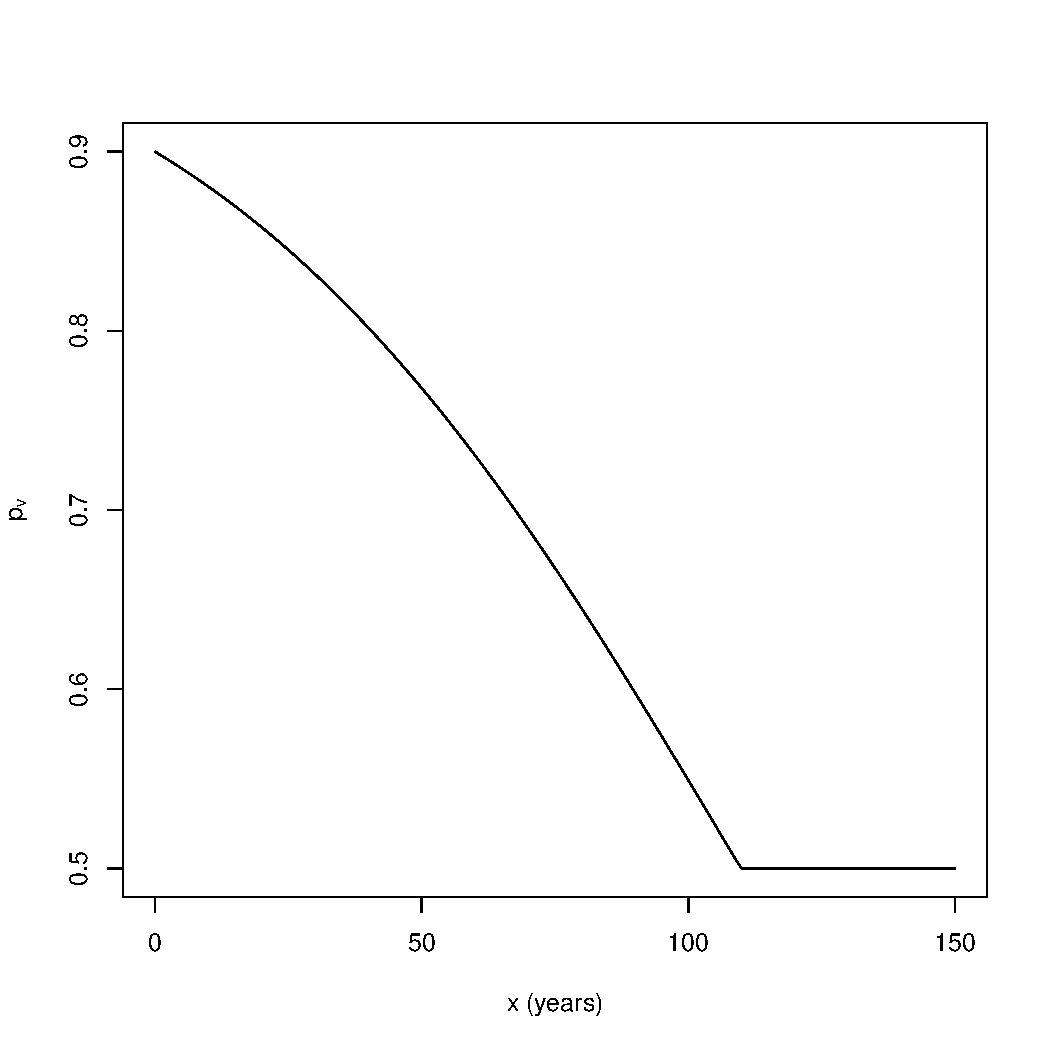
\includegraphics[scale=0.5]{figures/read-count-regr-1}
\caption{
Dependence of \(p_v\), the expected read fraction of the alternative allele,
on explanatory variable age \(x\) given by Eq.~\ref{eq:logit-p} when
\(\theta_{ig}=1\) (monoallelic expression) and the allele configuration is
\(\phi_{ig}=\psi_v\).  Regression parameter \(\beta_0 = \mathrm{logit}(p_1)\) where
\(p_1\) is fixed at \(0.9\).  \(\beta_1 = - 0.02 \, \mathrm{year}^{-1}\)
corresponding to an exponential decay time constant of \(50\) years.
}
\label{fig:Y-regression}
\end{center}
\end{figure}

\stepcounter{model}\subsection{Regression of \(\theta_{ig}\) on explanatory variables }
\label{sec:model-theta-regr}

We only sketch this regression model because~\ref{sec:model-Y-regr} looks a
better fitting candidate. Model~\ref{sec:model-theta-regr} is quite similar
to~\ref{sec:model-basic} (Figure~\ref{fig:theta-regression}). The key
difference is the replacement of \(\mu_g\) by \(x_i
\beta_{g}=(beta_{g0},...,\beta_{gR-1})\) so that the allelic state
\(\theta_{ig}\) is a response to the explanatory variables in \(x_i\) with
regression coefficient \(\beta_g\).  \(\beta_g\) in turn is a random variable
parametrized by vector \(\pi\) and some other parameters \(\rho\).  An
attractive distribution family is yet to be found for \(\beta_{gr}\).

\begin{figure}[t]
\begin{center}
\begin{tikzpicture}

\node[latent] (theta) {\(\theta_{ig}\)};
\factor[above=0.5 of theta, label=right:Multi]       {theta-f} {} {} {}; %
\node[latent, above=1.5 of theta, xshift=1 cm] (beta) {\(\beta_{gr}\)};
\node[const, above=1.5 of theta, xshift=-1 cm] (x) {\(x_i\)};
\factoredge {x, beta} {theta-f} {theta};

\factor[above=0.5 of beta]       {beta-f} {} {} {}; %
\node[latent, above=1.0 of beta, xshift=-0.75 cm] (pi) {\(\pi\)};
\node[latent, above=1.0 of beta, xshift=0.75 cm] (rho) {\(\rho\)};
\factoredge {pi, rho} {beta-f} {beta};

\plate {i-p} {(x) (theta)} {\(i=1,...,I\)} ;
\coordinate[below=0.75 of theta] (g-p-bottom) ;
\plate {g-p} {(theta) (beta) (g-p-bottom)} {\(g=1,...,G\)} ;

\plate {beta-p} {(beta)} {\(R\)} ;

\end{tikzpicture}
\end{center}
\caption{
The global structure of model~\ref{sec:model-theta-regr}.  The exclusion state
indicators \(\theta_{ig}\) play the role of response variables in regression.
Thus, the \(R-1\) explanatory variables in \(x_i\) have a direct effect on
exclusion state \(\theta_{ig}\) but only indirect effect on read counts
\(Y_v\).  This is the key distinction from the regression framework
of~\ref{sec:model-Y-regr}.
}
\label{fig:theta-regression}
\end{figure}

With this model structure the variation of exclusion state has three
components: the genome-wide variation of their effect mediated by \(\beta_g\),
a systematic within-gene variation due to the measured explanatory variables
\(x_i\), and the remaining within-gene variation unexplained by \(x_i\).

\renewcommand{\thesubsection}{\arabic{section}.\arabic{subsection}}
\section{Inference}
\label{sec:likelihood}

Likelihood functions play a central in both frequentist (classical) and
Bayesian inference.  In this section we present various likelihood functions
for the local and global models introduced in Section~\ref{sec:models}.

\subsection{Likelihood of local models}
\label{sec:likelihood-local}

Since the read count \(Y_v\) of the alternative variant at any given
heterozygous site \(v\), the lowest-level likelihood functions are
\begin{equation}
\label{eq:f-v-M1-M3}
\binom{n_v}{y_v} p_v^{y_v} (1-p_v)^{n_v-y_v}
=
\begin{cases}
f_v(y_v | n_v, P, \phi_{ig}, \psi_v, \theta_{ig}), & p_v =
\mathrm{Eq.~}\ref{eq:p-v-by-P-matrix}
\quad (\ref{sec:model-basic}, \ref{sec:model-theta-regr}) \\
f_v(y_v | n_v, x_i, B, \phi_{ig}, \psi_v, \theta_{g}), & p_v =
\mathrm{Eq.~}\ref{eq:logit-p},\ref{eq:logit-b-B}
\quad (\ref{sec:model-Y-regr}).
\end{cases}
\end{equation}

As mentioned in Section~\ref{sec:local-model} the allelic configurations \( \{
(\phi_{ig},\psi_v) : v\in(i,g) \} \) are neither observed nor informative and
so must be considered nuisance parameters to be removed by marginalization.
So we take the expectation over all possible configurations.  This yields the
following likelihood function under model~\ref{sec:model-basic}
and~\ref{sec:model-theta-regr}:
\begin{eqnarray}
\label{eq:f-ig}
L_{ig}^k &\equiv&
f_{ig}(y_{ig} | n_{ig}, P, \kappa, \theta_{ig}=k)
\\
\label{eq:f-ig-continued}
&=&
\frac{1}{2}
\sum_{\phi_{ig}=0}^1 \kappa^{\phi_v} (1 - \kappa)^{1-\phi_v}
\prod_{v\in(i,g)}
\sum_{\psi_v=0}^1
f_v(y_v | n_v, P, \phi_{ig}, \psi_v, \theta_{ig}=k),
\end{eqnarray}
where \(k=0,...,K-1\) and \(L_{ig}^k\) is a convenient shorthand.  Under
model~\ref{sec:model-Y-regr} \(f_{ig}\) has the same form except that \(P\) is
replaced by \(x_i,B\) and \(\theta_{ig}\) by \(\theta_g\) as in
Eq.~\ref{eq:f-v-M1-M3}.  The same shorthand \(L_{ig}^k\) shall
be used model~\ref{sec:model-Y-regr} as well; its specific semantics shall be clear from
the context.

\subsection{Regression parameters under~\ref{sec:model-Y-regr} from training data}
\label{sec:beta-from-training-data}

For this estimation we need a training set of genes known to be expressed
monoallelically (\(\theta_g=1\)), collected
from \(I'\) individuals.  Unless we have training data distinguishing between
different strengths of allelic exclusion, we must use the binary version of
model~\ref{sec:model-Y-regr}.  Then the likelihood for the \(B\) matrix of regression
parameters based on the training data is
\begin{eqnarray}
L_{\ref{sec:model-Y-regr}}(B) = \prod_{g} \prod_{i=1}^{I'} L_{ig}^1
%\sum_{\phi_{ig}=0}^1 \kappa^{\phi_v} (1 - \kappa)^{1-\phi_v}
%\prod_{v\in(i,g)}
%\binom{n_v}{y_v}
%\sum_{\psi_v=0}^1
%p_v^{y_v} (1-p_v)^{n_v-y_v},
\end{eqnarray}
where \(L_{ig}^1\) is given by the modification of
Eq.~\ref{eq:f-ig}-\ref{eq:f-ig-continued} as described in
Section~\ref{sec:likelihood-local}.  The two running products represent the
data aggregation over individuals \(i\) and monoallelically expressed genes
\(g\) describing the complete training data set.

\subsection{Model selection and estimation of \(\pi\)}
\label{sec:model-selection}

Consider a set \(\mathcal{M}\) of alternative models like the proposed ones in
this article.  Model selection means to find the best model(s) according to a
criterion reflecting its fit to the observed data.
The general frequentist\footnote{The presented frequentist model selection
procedure has a Bayesian
equivalent with the advantage that similarly well scoring models may be
averaged together. } procedure goes as follows:
\begin{enumerate}
\item
express the \emph{marginal likelihood} \(L_M\) for \(\pi\) based on \(y\)
and \(X\) under all models \(M\in \mathcal{M}\), by taking expectations (over nuisance
parameters such as \(\mu_{ig},\psi_v\) or over unknown \(\theta_{ig}\))
\item 
maximize \(L_M\) with respect to \(\pi\) obtaining the ML estimate
\(\hat{\pi}_M=\arg\max_\pi L_{M}(\pi)\)
\item for each \(M\in\mathcal{M}\) evaluate model fit using some objective,
likelihood-based, criterion such as AIC, BIC and select the highest scoring model
\(M^*\) and the corresponding \(\hat{\pi}_{M^*}\)
\end{enumerate}


In the following section (\ref{sec:marginal-likelihood-pi}) we will express
the marginal likelihoods for \(\pi\) (and possibly other parameters).
Computational points on optimization and implementation are not discussed.  In
Section~\ref{sec:simulation} we consider model comparison using simulated
data.

\subsubsection{Marginal likelihood}
\label{sec:marginal-likelihood-pi}

Under model~\ref{sec:model-basic} the marginal likelihood
\(L_{\ref{sec:model-basic}}(\pi,\nu)\equiv
f(y|n,P,\kappa,\pi,\nu)\) for \(\pi\) and \(\nu\) is given by

\begin{equation}
\label{eq:L-model-basic}
L_{\ref{sec:model-basic}}(\pi,\nu) =
%b^{-1}
\frac{\Gamma(\nu)}{\prod_k \Gamma(\pi_k\nu)}
\prod_{g} \int_{0}^{1} \prod_k \mu_k^{\pi_k\nu-1}
\prod_{i}
\sum_k L_{ig}^k
\, \mathrm{d}\mu.
\end{equation}

The summation of \(L_{ig}^k\) terms corresponds to taking expectation over all
\(K\) exclusion states, whereas the integral marginalizes over \(\mu\).  The
running product over \(i\) follows from the conditional independence of
exclusion states among individuals given gene \(g\), and the one over \(g\)
from the assumed independence of genes.

\(L_{\ref{sec:model-basic}}\) in Eq.~\ref{eq:L-model-basic} depends on the parameter \(\nu\), which
may be of some interest because it quantifies the population-wide variation of
exclusion state within any given gene.  We may decide not to care about \(\nu\) or take
it to the limit \(\nu\rightarrow 0\) or \(\nu\rightarrow \infty\) by
choosing~\ref{sec:model-basic-nu-0} or~\ref{sec:model-basic-nu-infinit} a
priori, i.e.~without evaluating how well they fit the data.  To obtain the
likelihood for those cases let us denote \(L_{\ref{sec:model-basic}}(\pi)\equiv
f(y|n,p,\kappa,\pi)\) and recall Eq~\ref{eq:f-ig}.  Then
Eq.~\ref{eq:L-model-basic} simplifies to
\begin{eqnarray}
\label{eq:L-model-basic-nu-0}
L_{\ref{sec:model-basic-nu-0}}(\pi) &=&
\prod_{g}
\sum_k \prod_i L_{ig}^k
\\
\label{eq:L-model-basic-nu-infinit}
L_{\ref{sec:model-basic-nu-infinit}}(\pi) &=&
\prod_{i,g}
\sum_k L_{ig}^k,
\end{eqnarray}
where \(L_{ig}^k\) is used in the sense of
\ref{sec:model-basic}-\ref{sec:model-theta-regr} (Eq.~\ref{eq:f-ig}).

Turning to model~\ref{sec:model-Y-regr}, let us assume that the matrix \(B\)
of regression parameters is known (preset and/or estimated as in
Section~\ref{sec:beta-from-training-data}).  Write
\(L_{\ref{sec:model-Y-regr}}(\pi)\equiv f(y|n,X,B,\kappa,\pi)\).  It is easy
to see that \(L_{\ref{sec:model-Y-regr}}(\pi)\) has the same form as
Eq.~\ref{eq:L-model-basic-nu-0}; of course in this case the semantics of
\(L_{ig}^k\) is connected to \ref{sec:model-Y-regr} (recall remark below
Eq.~\ref{eq:f-ig}-\ref{eq:f-ig-continued}).

\subsection{Classification}
\label{sec:classification}

For binary exclusion state (\(K=2\)) we can
formulate the task of classification for a given \((i,g)\) as the statistical test of two simple
hypotheses.  The null hypothesis is that of biallelic expression: \(B_{ig} :\;
\theta_{ig}=0\) and the alternative monoallelic expresssion \(M_{ig} :\; \theta_{ig}=1\).

As mentioned in Section~\ref{sec:improvement} the Neyman-Pearson lemma ensures
that the likelihood ratio \(\Lambda_{ig}=L_{ig}^1/L_{ig}^0\) used as test
statistic affords the most powerful test at a given significance level, so it
is highly preferable to use \(\Lambda_{ig}\).  For nested hypotheses
\(H_0\subset H_1\) the asymptotic distribution of twice the log-likelihood
ratio is \(\chi^2\) with degrees of freedom given by the increase in unknown
parameters from \(H_0\) to \(H_1\).  However, in the present case
\(H_0=B_{ig}\) and \(H_1=M_{ig}\) because we defined exclusion states based on
disjoint intervals (\(\mathcal{P}_0\) and \(\mathcal{P}_1\),
Section~\ref{sec:local-binary}).  For this reason \(H_0\) is not \(\subset H_1\)
so the asymptotic \(\chi^2\) distribution doesn't hold.

Fortunately, however, the present case lends itself to Bayesian hypothesis
testing with \(\Lambda_{ig}\) playing the role of Bayes factor and
\(\pi_1/\pi_0\) the corresponding prior odds.  Let's write
\(\mathrm{Pr}(M_{ig})\equiv\pi_1\) to emphasize that \(\pi_1\) is the prior
probability of monoallelic expression. Likewise, let
\(\mathrm{Pr}(B_{ig})\equiv\pi_0\).  Then the posterior probability of
monoallelic expression given \(n_{ig}\) and after observing that
\(Y_{ig}=y_{ig}\) is
\begin{equation}
\label{eq:hypothesis-posterior}
\mathrm{Pr}(M_{ig}|n_{ig},y_{ig}) =
\frac{L_{ig}^1 \mathrm{Pr}(M_{ig})}{{L_{ig}^1 \mathrm{Pr}(M_{ig})} + {L_{ig}^0
\mathrm{Pr}(B_{ig})}}.
\end{equation}

This Bayesian hypothesis testing easily extends to the general case of
\(K\)-ary allelic state (\(K\ge 2\)), where \(B_{ig} :\;
\theta_{ig}=0\) as in the binary case but \(M_{ig}: \theta_{ig}>0\).  Then
\(\mathrm{Pr}(\theta_{ig}=k)\) can be calculated as
\(
%\mathrm{Pr}(\theta_{ig}=k|n_{ig},y_{ig}) =
L_{ig}^1 \mathrm{Pr}(\theta_{ig}=k)
\big/
\sum_{k'} L_{ig}^{k'} \mathrm{Pr}(\theta_{ig}={k'})
\).  Therefore \(\mathrm{Pr}(M_{ig}|n_{ig},y_{ig}) = \sum_{k:k>0}
\mathrm{Pr}(\theta_{ig}=k)\).

\subsection{Thoughts on simulations}
\label{sec:simulation}

Simulations are helpful in many ways such as comparing performance of alternative approaches in
some inference task.  Two important choices must be made prior to a
simulation experiment: the inference task and the model (the sampling
distribution).  Testing under all relevant tasks (classification or estimation of parameters
such as \(\pi\)) is desirable.  However, a single model that presumed to be true should be selected based on mechanistic arguments and/or model fit to
real data.

In the present case, what should be that presumed true model?  As pointed out
in Section~\ref{sec:improvement}, the previous approaches do not allow
objective, likelihood-based, evaluation of model fit.  Turning to mechanistic
arguments, how should allelic exclusion depend on the measured explanatory
variables like age or gender?  Suppose we have a reason to exclude such
dependence.  Then it still remains to be specified how allelic exclusion
varies population-wide within any given gene.

\end{document}
